\section*{Einleitung}

Die Anzahl an Smartphone Nutzern wächst stetig und der Markt der mobilen Betriebssysteme bildet im Wesentlichen zwei Gruppen: Android und iOS~\cite{statista}.
Anwendungen die für das eine System entwickelt wurden, sind aber nicht mit dem anderen kompatibel.
So sind Android Apps typischerweise in Java geschrieben und Zugriffe auf die nativen Gerätekomponenten laufen über Androids API Frameworks.
Im Gegensatz dazu werden iOS Anwendungen in Swift entwickelt und nutzen die Apple eigenen Schnittstellen für Hardwarezugriffe.
Um jedoch möglichst viele Nutzer erreichen zu können, müssen mobile Anwendungen für beide Plattformen bereitgestellt werden. Unternehmen und Entwickler stehen folglich vor der Herausforderung ein und dieselbe App für zwei grundsätzlich verschiedene Systeme bauen zu müssen.
Das bedeutet doppelter Aufwand beim Gestalten, Entwickeln der Funktionalität und Logik, Testen und Warten der Anwendung. \\ \\
Diesem Problem nehmen sich cross-plattform Lösungen an. Sie ermöglichen es, statt jeweils eine Anwendung für iOS und Android entwickeln zu müssen, aus dem selben Sourcecode sowohl eine native Android als auch iOS App zu bauen.
Es existieren bereits viele solcher Technologien. In dem Paper “Evaluating Cross-Platform Development Approaches for Mobile Applications” von Heitkötter, Hanschke und Majchrzak aus dem Jahr 2012 vergleichen die Autoren damalige Ansätze zur cross-plattform Entwicklung mobiler Anwendungen~\cite{eva12}.
Seit dem haben sich die dort betrachteten Tools zum einen weiterentwickelt, zum anderen sind weitere hinzugekommen. So ist jetzt auch Google in diesen Markt eingetreten und stellt derzeit das Flutter SDK vor~\cite{flutter}. \\ \\
Es gibt bislang sehr wenig Forschung zu aktuellen cross-platform Lösungen. Aber durch den kontinuierlichen Zuwachs an Tools wird es für Unternehmen und Entwickler zunehmend herausfordernder, den Überblick zu behalten und eine passende Technologie zu wählen. Diese Arbeit soll dabei unterstützen und nimmt sich daher der nachfolgenden Frage an:

\section*{Fragestellung}

Wo liegen die Stärken und Schwächen aktueller cross-platform Lösungen zur Entwicklung mobiler Anwendungen?

\section*{Methodik}

Diese Bachelorarbeit baut auf das oben genannte Paper “Evaluating Cross-Platform Development Approaches for Mobile Applications” von Heitkötter, Hanschke und Majchrzak auf. Die Autoren unterteilen zunächst damalig aktuelle cross-platform Lösungen zur Entwicklung mobiler Anwendungen in drei Gruppen:
\begin{itemize}
    \item Web Apps sind Anwendungen, die vollständig im Browser des Smartphones laufen. Sie sind größtenteils mit JavaScript, HTML, CSS und zusätzlichse Web Frameworks entwickelt und unterscheiden sich heutzutage von responsiven Webseiten unwesentlich~\cite{eva12}.
    Beispielhafte Frameworks sind jQuery Mobile~\cite{jquery} oder das mittlerweile in Sencha Ext JS integrierte Sencha Touch~\cite{sencha}.
    Auch Progressive Web Apps (PWAs) fallen in diese Kategorie, da sie ausschließlich vom Browser ausgeführt werden.
    Durch die zahlreichen Anbindungen moderner Browser an Smartphonesensoren wie Kamera oder GPS und die Möglichkeit Push-Benachrichtigungen sowie Offline-Funktionalität durch den Einsatz von Service Workern umzusetzen, haben PWAs große Überschneidungen mit Anwendungen der zweiten Kategorie (hybride Apps)~\cite{pwa}.
    
    \item Hybride Apps bilden die Brücke zwischen nativen Anwendungen und Web Apps. Die Laufzeitumgebung hybrider Apps besteht aus einer für das Layout und Rendering zuständige Browser-Engine, welche für hardwarespezifische Zugriffe in eine native Engine eingebettet ist~\cite{eva12}.
    Mobile Browser sind jedoch in den letzten Jahren zunehmend mächtiger geworden, womit sich auch der Funktionsumfang von reinen Web Apps enorm erweitern lässt~\cite{gdev}.
    Bekannte Beispiele für hybride Lösungen sind PhoneGap oder das Ionic Framework~\cite{phonegap,ionic}.
    
    \item Apps, die vollständig In sich geschlossene Laufzeitumgebung (self-contained Apps) eigene Engine ... TODO
\end{itemize}
Aus jeder dieser Gruppen wählen sie eine der Lösungen als Repräsentant und untersuchen diesen anhand eigens aufgestellter Kriterien. Die Auswahl dieser Kriterien basiert auf Interviews mit Fachexperten, Literaturrecherche, typischen Problemen in Webforen und eigenen Erfahrungen beim Entwickeln prototypischer Apps. Diese Kriterien bilden die Grundlage weiterer Arbeiten wie beispielsweise “A Comparative Analysis of Cross-platform Development Approaches for Mobile Applications” von Xanthopoulos und Xinogalos aus dem Jahr 2013~\cite{compa13}.
Pro Kriterium wird jeder Ansatz von 1 (Kriterium wurde sehr gut erfüllt) bis 6 (Kriterium wurde gar nicht bzw. sehr schlecht erfüllt) bewertet. Die Bewertung stützt sich sowohl auf aus Interviews gewonnenen Einschätzungen erfahrener Entwickler, als auch Literaturrecherche und praktischen Erfahrungen, die die Autoren beim Arbeiten mit der jeweiligen Technologie selber gesammelt haben.\\ \\
Die Methodik dieser Bachelorarbeit orientiert sich am Vorgehen der Arbeit von Heitkötter, Hanschke und Majchrzak. Zunächst werden überblicksartig derzeit aktuelle cross-platform Lösungen vorgestellt und jeweils einer der drei oben genannten Gruppen zugeordnet. Anschließend wird aus jeder Gruppe ein Repräsentant ausgewählt und anhand der Kriterien des zugrundeliegenden Papers untersucht. Abschließend werden die Ergebnisse ausgewertet und tabellarisch gegenübergestellt, um die Stärken und Schwächen der jeweiligen Lösung aufzuzeigen und so Entwickler bei der Wahl einer passenden Technologie zu unterstützen.

\section*{Vorläufige Gliederung}

\begin{enumerate}
\item Einleitung
\begin{enumerate}[label*=\arabic*.]
\item Motivation, Fragestellung, Methodik
\end{enumerate}
\item Stand der Forschung
\begin{enumerate}[label*=\arabic*.]
\item Vorstellung der zugrundeliegenden Arbeit
\end{enumerate}
\item Überblick aktueller cross-platform Lösungen
\begin{enumerate}[label*=\arabic*.]
\item Klassifizierung der Lösungen
\end{enumerate}
\item Untersuchung der Lösungen anhand der Kriterien der zugrundeliegenden Arbeit
\item Auswertung der Ergebnisse
\item Fazit 
\end{enumerate}

 \section*{Zeitplan}
 \begin{figure}[H]
	\renewcommand*\figurename{Abbildung}
		\begin{center}
			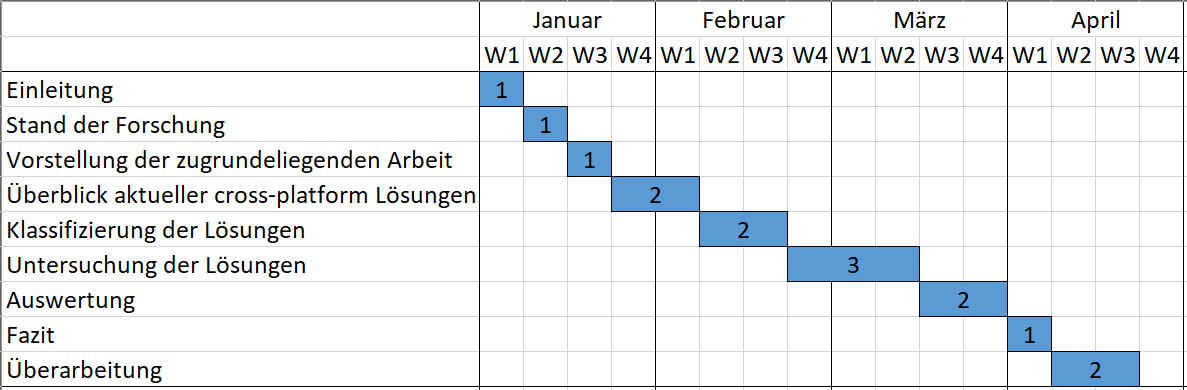
\includegraphics[width=1\textwidth]{timetable.png}
		\end{center}
		\caption{Zeitliche Gliederung der Bachelorarbeit}
	\end{figure}